\documentclass[
	% -- opções da classe memoir --
	12pt,				% tamanho da fonte
	openright,			% capítulos começam em pág ímpar (insere página vazia caso preciso)
	%twoside,			% para impressão em recto e verso. Oposto a oneside
	oneside,      % para impressão direta das páginas. Oposto a twoside
	a4paper,			% tamanho do papel.
	% -- opções da classe abntex2 --
	%chapter=TITLE,		% títulos de capítulos convertidos em letras maiúsculas
	%section=TITLE,		% títulos de seções convertidos em letras maiúsculas
	%subsection=TITLE,	% títulos de subseções convertidos em letras maiúsculas
	%subsubsection=TITLE,% títulos de subsubseções convertidos em letras maiúsculas
	% -- opções do pacote babel --
	english,			% idioma adicional para hifenização
	french,				% idioma adicional para hifenização
	spanish,			% idioma adicional para hifenização
	brazil,				% o último idioma é o principal do documento
	]{abntex2}\usepackage[]{graphicx}\usepackage[table]{xcolor}
% maxwidth is the original width if it is less than linewidth
% otherwise use linewidth (to make sure the graphics do not exceed the margin)
\makeatletter
\def\maxwidth{ %
  \ifdim\Gin@nat@width>\linewidth
    \linewidth
  \else
    \Gin@nat@width
  \fi
}
\makeatother

\definecolor{fgcolor}{rgb}{0.345, 0.345, 0.345}
\newcommand{\hlnum}[1]{\textcolor[rgb]{0.686,0.059,0.569}{#1}}%
\newcommand{\hlstr}[1]{\textcolor[rgb]{0.192,0.494,0.8}{#1}}%
\newcommand{\hlcom}[1]{\textcolor[rgb]{0.678,0.584,0.686}{\textit{#1}}}%
\newcommand{\hlopt}[1]{\textcolor[rgb]{0,0,0}{#1}}%
\newcommand{\hlstd}[1]{\textcolor[rgb]{0.345,0.345,0.345}{#1}}%
\newcommand{\hlkwa}[1]{\textcolor[rgb]{0.161,0.373,0.58}{\textbf{#1}}}%
\newcommand{\hlkwb}[1]{\textcolor[rgb]{0.69,0.353,0.396}{#1}}%
\newcommand{\hlkwc}[1]{\textcolor[rgb]{0.333,0.667,0.333}{#1}}%
\newcommand{\hlkwd}[1]{\textcolor[rgb]{0.737,0.353,0.396}{\textbf{#1}}}%
\let\hlipl\hlkwb

\usepackage{framed}
\makeatletter
\newenvironment{kframe}{%
 \def\at@end@of@kframe{}%
 \ifinner\ifhmode%
  \def\at@end@of@kframe{\end{minipage}}%
  \begin{minipage}{\columnwidth}%
 \fi\fi%
 \def\FrameCommand##1{\hskip\@totalleftmargin \hskip-\fboxsep
 \colorbox{shadecolor}{##1}\hskip-\fboxsep
     % There is no \\@totalrightmargin, so:
     \hskip-\linewidth \hskip-\@totalleftmargin \hskip\columnwidth}%
 \MakeFramed {\advance\hsize-\width
   \@totalleftmargin\z@ \linewidth\hsize
   \@setminipage}}%
 {\par\unskip\endMakeFramed%
 \at@end@of@kframe}
\makeatother

\definecolor{shadecolor}{rgb}{.97, .97, .97}
\definecolor{messagecolor}{rgb}{0, 0, 0}
\definecolor{warningcolor}{rgb}{1, 0, 1}
\definecolor{errorcolor}{rgb}{1, 0, 0}
\newenvironment{knitrout}{}{} % an empty environment to be redefined in TeX

\usepackage{alltt}

% ---
% PACOTES
% ---

% ---
% Pacotes fundamentais
% ---
\usepackage{lmodern}			% Usa a fonte Latin Modern
\usepackage[T1]{fontenc}		% Selecao de codigos de fonte.
\usepackage[utf8]{inputenc}		% Codificacao do documento (conversão automática dos acentos)
\usepackage{indentfirst}		% Indenta o primeiro parágrafo de cada seção.
\usepackage{color}				% Controle das cores
\usepackage{graphicx}			% Inclusão de gráficos
\usepackage{microtype} 			% para melhorias de justificação
% ---
\usepackage{booktabs}
\usepackage[table]{xcolor}
\usepackage{amssymb}
\usepackage{amsthm}
\usepackage{amsmath}
\usepackage{float}
\usepackage{here}
\usepackage{listings}
\usepackage{booktabs}

\usepackage{xcolor}

%New colors defined below
\definecolor{codegreen}{rgb}{0,0.6,0}
\definecolor{codegray}{rgb}{0.5,0.5,0.5}
\definecolor{codepurple}{rgb}{0.58,0,0.82}
\definecolor{backcolour}{rgb}{0.95,0.95,0.92}



\lstdefinestyle{mystyle}{
  backgroundcolor=\color{backcolour}, commentstyle=\color{codegreen},
  keywordstyle=\color{magenta},
  numberstyle=\tiny\color{codegray},
  stringstyle=\color{codepurple},
  basicstyle=\ttfamily\footnotesize,
  breakatwhitespace=false,         
  breaklines=true,                 
  captionpos=b,                    
  keepspaces=true,                 
  numbers=left,                    
  numbersep=5pt,                  
  showspaces=false,                
  showstringspaces=false,
  showtabs=false,                  
  tabsize=2
}

%"mystyle" code listing set
\lstset{style=mystyle}


% ---
% Pacotes adicionais, usados apenas no âmbito do Modelo Canônico do abnteX2
% ---
\usepackage{lipsum}				% para geração de dummy text
% ---
\theoremstyle{definition}
\newtheorem{definition}{Definição}[section]
% ---
% Pacotes de citações
% ---
\usepackage[brazilian,hyperpageref]{backref}	 % Paginas com as citações na bibl
\usepackage[alf]{abntex2cite}	% Citações padrão ABNT

% ---
% CONFIGURAÇÕES DE PACOTES
% ---

% ---
% Configurações do pacote backref
% Usado sem a opção hyperpageref de backref
\renewcommand{\backrefpagesname}{Citado na(s) página(s):~}
% Texto padrão antes do número das páginas
\renewcommand{\backref}{}
% Define os textos da citação
\renewcommand*{\backrefalt}[4]{
	\ifcase #1 %
		Nenhuma citação no texto.%
	\or
		Citado na página #2.%
	\else
		Citado #1 vezes nas páginas #2.%
	\fi}%
% ---

% ---
% Informações de dados para CAPA e FOLHA DE ROSTO
% ---
\titulo{Modelo de Regressão Logística Aplicada a Previsão de Inadimplência sobre Cartão de Crédito de uma Instituição Financeira}
\autor{DOUGLAS VINÍCIUS GONÇALVES ARAÚJO}
\local{JI-PARANÁ}
\data{2023}
\instituicao{%
  UNIVERSIDADE FEDERAL DE RONDÔNIA -- UNIR
  \par
  DEPARTAMENTO DE MATEMÁTICA E ESTATÍSTICA
  \par
  RELATÓRIO DE PESQUISA}
\tipotrabalho{Tese (Doutorado)}
% O preambulo deve conter o tipo do trabalho, o objetivo,
% o nome da instituição e a área de concentração
\preambulo{Relatório de Estágio Supervisionado apresentado como Trabalho de Pesquisa à Coordenação do Curso de Bacharelado em Estatística da Universidade Federal de Rondônia.}
% ---

% ---
% Configurações de aparência do PDF final

% alterando o aspecto da cor azul
\definecolor{blue}{RGB}{41,5,195}

% informações do PDF
\makeatletter
\hypersetup{
     	%pagebackref=true,
		pdftitle={\@title},
		pdfauthor={\@author},
    	pdfsubject={\imprimirpreambulo},
	    pdfcreator={LaTeX with abnTeX2},
		pdfkeywords={abnt}{latex}{abntex}{abntex2}{projeto de pesquisa},
		colorlinks=true,       		% false: boxed links; true: colored links
    	linkcolor=blue,          	% color of internal links
    	citecolor=blue,        		% color of links to bibliography
    	filecolor=magenta,      		% color of file links
		urlcolor=blue,
		bookmarksdepth=4
}
\makeatother
% ---

% ---
% Espaçamentos entre linhas e parágrafos
% ---

% O tamanho do parágrafo é dado por:
\setlength{\parindent}{1.3cm}

% Controle do espaçamento entre um parágrafo e outro:
\setlength{\parskip}{0.2cm}  % tente também \onelineskip

% ---
% compila o indice
% ---
\makeindex
% ---

% ----
% Início do documento
% ----
\IfFileExists{upquote.sty}{\usepackage{upquote}}{}
\begin{document}

% Seleciona o idioma do documento (conforme pacotes do babel)
%\selectlanguage{english}
\selectlanguage{brazil}

% Retira espaço extra obsoleto entre as frases.
\frenchspacing

% ----------------------------------------------------------
% ELEMENTOS PRÉ-TEXTUAIS
% ----------------------------------------------------------
% \pretextual

% ---
% Capa
% ---
\imprimircapa
% ---

% ---
% Folha de rosto
% ---
\imprimirfolhaderosto
% ---
\clearpage
% ---
% NOTA DA ABNT NBR 15287:2011, p. 4:
%  ``Se exigido pela entidade, apresentar os dados curriculares do autor em
%     folha ou página distinta após a folha de rosto.''
% ---
%\begin{agradecimentos} 
%  Os agradecimentos... 
%\end{agradecimentos}
% ---
% Epígrafe

\begin{epigrafe} 
  \vspace*{\fill} 
  \begin{flushright} 
  \textit{"Os livros servem para nos lembrar quanto somos estúpidos e tolos. 
      \\ São o guarda pretoriano de César, cochichando enquanto o desfile ruge 
      \\ pela avenida: – Lembre-se, César, tu és mortal. A maioria de nós não 
      \\ pode sair correndo por aí, falar com todo mundo, conhecer todas as 
      \\ cidades do mundo, não temos tempo, dinheiro ou tantos amigos assim. 
      \\ As coisas que você está procurando, Montag, estão no mundo, mas a 
      \\ única possibilidade que o sujeito comum terá de ver noventa e nove 
      \\ por cento delas está num livro". 
      \\ - Fahrenheit 451 de Ray Douglas Bradbury} 
  \end{flushright} 
\end{epigrafe}
% ---

% --- resumo em português--
\begin{resumo} 
  O objetivo deste trabalho tem como aplicar uma análise de regressão logística a dados
  de cartões de crédito de uma instituição financeira do estado de Rondônia, de forma
  gerar um modelo logístico capaz de prever a probabilidade de inadimplência ou risco
  de o tomador não honrar com o crédito.
  \vspace{\onelineskip} 
  \noindent
  
  \textbf{Palavras-chaves}: Credit Scoring, Machine Learning, Probabilidade de Default, Regressão Logístico. 
\end{resumo}

% ---
% inserir lista de ilustrações
% ---
\pdfbookmark[0]{\listfigurename}{lof}
\listoffigures*
\cleardoublepage
% ---

% ---
% inserir lista de tabelas
% ---
\pdfbookmark[0]{\listtablename}{lot}
\listoftables*
\cleardoublepage
% ---

% ---
% inserir lista de abreviaturas e siglas
% ---
%\begin{siglas}
%  \item[ABNT] Associação Brasileira de Normas Técnicas
%  \item[abnTeX] ABsurdas Normas para TeX
%\end{siglas}
% ---

% ---
% inserir lista de símbolos
% ---
%\begin{simbolos}
%  \item[$ \Gamma $] Letra grega Gama
%  \item[$ \Lambda $] Lambda
%  \item[$ \zeta $] Letra grega minúscula zeta
%  \item[$ f(x;\theta)$] Função de Densidade de Probabilidade
%  \item[$ \Pi $] Produtório
%\end{simbolos}
% ---

% ---
% inserir o sumario
% ---
\pdfbookmark[0]{\contentsname}{toc}
\tableofcontents*
\cleardoublepage
% ---

% ----------------------------------------------------------
% ELEMENTOS TEXTUAIS
% ----------------------------------------------------------
\textual

% ----------------------------------------------------------
% Introdução
% ----------------------------------------------------------
\chapter[Introdução]{Introdução}
%\addcontentsline{toc}{chapter}{INTRODUÇÃO}

A economia em crescimento trás consigo a expansão das linhas de créditos oferecidas pelas instituições financeiras.
E umas dessas linhas de créditos oferecidas, conhecemos pelo nome de cartão de crédito. Cartão de crédito em resumo, é uma forma de empréstimos com prazo de até 40 dias, disponível para fazer compras de bens e serviços. As taxas normalmente são padrão entre os bancos, mas o limite é definido com base na renda do solicitante do produto bancário.

Desta forma, torna-se mais importante para as instituições entender melhor os seus clientes para melhor oferecer as concessões de créditos e manter uma carteira de crédito bem gerida, evitar grandes prejuízos.





  \section{Objetivos}

A presente pesquisa é desenvolver um modelo de previsão de risco de inadimplência dos tomadores de cartões de créditos de uma instituição Financeira do Estado de Rondônia. Resumidamente, estamos interessados em construir um modelo preditivo de uma amostra de trainamento e após verificar a eficência deste modelo em uma amostra teste. Este modelo propõe auxiliar na tomada de decisão sobre o risco de crédito (ou modelo de Credit Scoring) das concessões de cartões de créditos.

Em todo processo de tomada de decisão pareamos entre duas hipotéses possíveis, podendo-se cometer dois tipos de erros. Um é recusar a concessão de crédito de um solicitante que, apesar de ter um perfil de alto risco, honraria seu compromisso. Outro erro é oferecer o crédito ao solicitante que irá implicar me perdas no futuro. Portanto, é ideal que temos um modelo eficaz para minizar esses erros.

Neste contexto, vamos relacionar os seguintes objetivos específicos:

\begin{itemize}
  \item Implementar um modelo de \textit{Credit Scoring} por meio de Regressão Logística;
  \item 
  \item 
\end{itemize}


% ----------------------------------------------------------
% Capitulo de textual
% ----------------------------------------------------------
\chapter{REFERENCIAL TEÓRICO}


  \section{Credit Scoring}
  
Segundo \cite{sicsu2010credit}, inúmeras tomadas de decisões precede a incertezas, com a concessão de crédito não se destingui disto, conceder crédito implica a possibilidade de perda. Razão está que o 
credor ao estimar a probabilidade de perda ajudará na sua tomada de decisão mais confiável. E este modelo de estimação chamado de credit scoring tem como objetivo de prever ou quantificar, na data da concessão de crédito, a probabilidade de perda em uma operação de crédito que denominanos \textbf{risco de crédito}. 
  
  
  
  
  \section{Breve Introdução sobre Machine Learning}
  
Uma definição básica sobre Machine Learning (Aprendizado de Máquina) é englobar 
um conjunto de regras com algoritmos e procedimentos que tem como objetivo de 
extrair informações apartir dos dados e dessas informações tomar uma decisão.

Segundo \cite{goodfellow2016deep}, os algoritmos de Machine Learning podem ser 
amplamente categorizados pelos tipos de aprendizagem, sitentizando essas diferenças
no tipo de experiência durante o aprendizado do algoritmo.

    \begin{figure}
      \caption{\label{img1}Machine Learning e suas aplicações}
      \begin{center}
        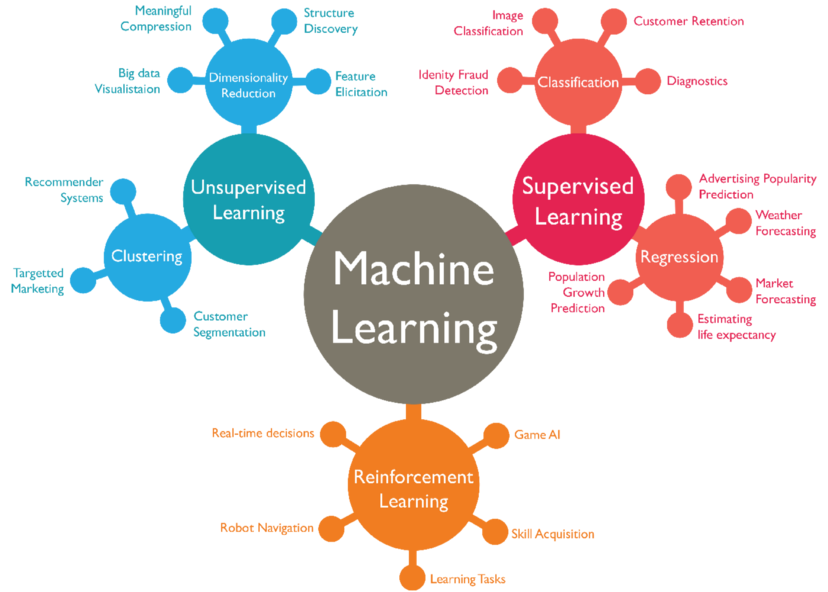
\includegraphics[scale = 0.4]{image/img1.png}
      \end{center}
      \legend{Fonte: \citeonline{machine22}}
    \end{figure}
  
\begin{itemize}
  \item Supervisionado: O algoritmo procura relação entre as variáveis preditoras e 
  a variável resposta de um \textit{dataset}. Através dessas associação é possível 
  realizar previsões quando o algoritmo é apresentado novos dados;
  \item Não-Supervisionado: aqui o algoritmo tem como objetivo agrupar os dados com 
  base em características similares, descartando à apresentação da variavél resposta ao 
  algoritmo;
  \item Aprendizagem por reforço: o algoritmo aprende com base nas interações com o 
  ambiente. Não são apresentadas as ações que devem ser tomadas, apenas as consequências das ações.
\end{itemize}

A Figura \ref{img1} representa a composição da área de \textit{machine learning} com as devidas
técnicas utilizadas para aprendizagem.


  \section{Modelo de Regressão Logística}

  
A regressão logística tem como principal uso, modelar uma variável binária $(0,1)$,
com base em mais variáveis, estas chamadas de variáveis explicativas ou preditoras.
E comumentemente a variável resposta ou dependente, assim chama-se a variável
binária do modelo. Conforme \cite{hilbe2016practical}, o melhor modelo ajustado 
aos dados é assumido que:
\begin{itemize}
  \item Não há correlação entre as variáveis preditoras;
  \item Estejam significativamente relacionados com a resposta;
  \item Que as observações dos dados não interferem entre si.
\end{itemize}
  
A resposta do modelo dito está conveniente a uma distribuição subjacente, ou seja,
segue uma distribuição de Bernoulli. Concordantemente com \cite{bolfarine2010introduccao}, 
esta distribuição é um distribuição particular da distribuição Binomial que 
a função de probabilidade pode ser expressa:
\begin{equation}\label{bernoulli}
  f(x;\theta) = \theta_{i}^{x_i}(1 - \theta_{i})^{1 - x_i}, \quad x_i = 0,1,
\end{equation}

\noindent em que $i = 1,\cdots,n$. Estes modelos são comumente empregados em situações
que a resposta é dicotômica.

\begin{comment}
Porque não utilizar o modelo de regressão linear? Suponhamos uma situação, estamos 
tentando prever a condição médica de um paciente com três diagnósticos possíveis: 
acidente vascular cerebral (AVC), overdose de drogas e convulsões epilépticas. 
Podemos dar a essas condições valores como uma variável de resposta quantitativa:

$$Y = \left\{
\begin{array}{rcl}
1, & \textrm{se AVC}\\
2, & \textrm{se overdose}\\
3, & \textrm{se convulsões}
\end{array}
\right.$$

Com essa converssão implica um ordenação dos resultados possíveis de $Y$, mas 
não há ordenação, pois se houvesse um ordenamento natural de leve, moderado e 
grave, da consideração a diferença de leve a moderado e entre moderado e grave 
seriam semelhantes os intervalos. Infelizmente, em geral, não há uma maneira de converter
uma variável resposta qualitativa com mais de dois níveis em uma resposta quantitativa 
pronta para regressão linear.

Se tivermos uma resposta qualitativa binária (dois níveis), por exemplo, duas condições
médicas do paciente e utilizando a variável \textit{dummy} para codificar a resposta:

$$
Y = \left\{
\begin{array}{rcl}
1, & \textrm{se AVC}\\
2, & \textrm{se overdose}
\end{array}
\right.
$$

\end{comment}

Mesmo usando a regressão linear para utilizar para obter uma estimativa de probabilidade
do resultado, quebramos um pressuposto, pois algumas estimativas podem estar fora do
intervalo $[0,1]$. Pois está expressão acarreta que é possível para $E(Y|x)$ assumir qualquer valor. 

Presuma que o modelo linear tradicional tenha a forma: 

\begin{equation}
  y_{i} = \mathbf{x'}_i \beta + \varepsilon_i
\end{equation}

\noindent em que $\mathbf{x'}_i = [1,x_{i1},x_{i2},\cdots,x_{ik}]$, $\beta' = 
[\beta_0,\beta_1,\beta_2,\cdots,\beta_k]$ e a variável resposta tem valores entre
o intervalo $[0,1]$. 


Assumiremos qeu a variável resposta é uma variável aleatória 
com distribuição de Bernoulli com função de probabilidade dita anteriormente pela 
equação \ref{bernoulli}.

Uma vez que a $E(\varepsilon_i) = 0$, o valor esperado da variável resposta é:
\begin{equation}
  E(y_i) = 1(\pi_i) + 0(1 - \pi_i)= \pi_i
\end{equation}

\noindent o que implica em $E(y_i) = \mathbf{x_i'}\beta = \pi_i$, ou seja, o valor esperado da função
resposta é apenas a probabilidade de que a variável resposta assuma o valor $1$. Como o nosso valor esperado é $\pi_i$ e o resultado dicotômico da variável deve ser maior ou igual a zero e menor do que um ($0 \leq E(y_i) = \pi_i \leq 1$). Pode ser visto na Figura \ref{img2} que a curva é em forma de "S" e se assemelhace a um gráfico 





    \begin{figure}
      \caption{\label{img2}Gráfico do modelo de regressão logística.}
      \begin{center}
        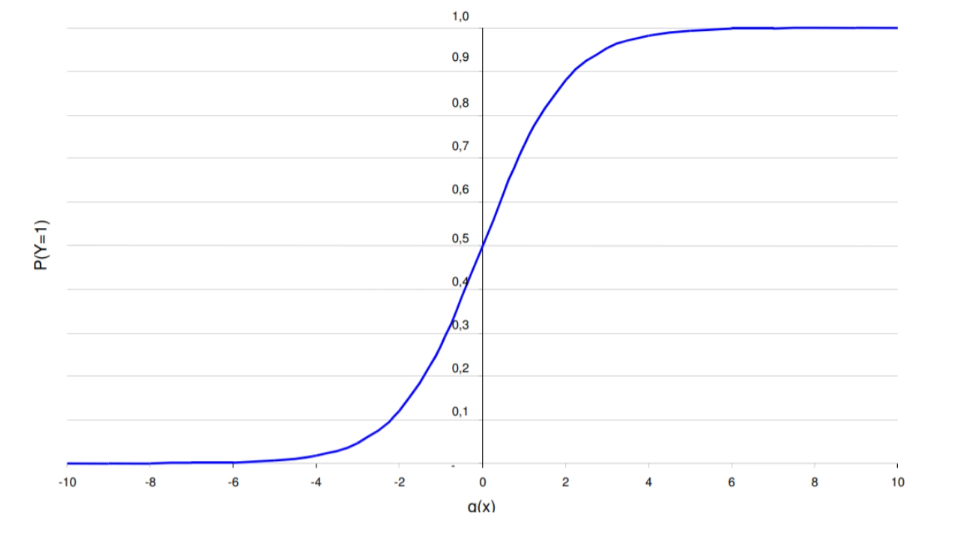
\includegraphics[scale = 0.6]{image/img2.png}
      \end{center}
      \legend{Fonte: https://aprenderdatascience.com/regressao-logistica/}
    \end{figure}


    \section{Estimação dos Parâmetros}
    
Para que se tenha um modelo ajustado, é imprescedível que seja feito a estimação dos parâmetros da regressão. Com isso utiliza-se o método de estimação de máxima de verossimilhança. Este método, a partir de um conjunto e um modelo estatístico, estima os valores dos parâmetros do modelo que mais máxima a probabilidade dos dados observados, ou seja, busca parâmetros que maximizem a função de verossimilhança. Condizente \cite{bolfarine2010introduccao}, a definição da função de verossimilhança é:

\begin{definition}{Definição}
    Sejam $X_1,\ldots,X_n$ uma amostra aleatória de tamanho $n$ da variável aleatória $X$ com função densidade $f(x|\theta)$, com $\theta \in \Theta$ é o espaço paramétrico. A função de verossimilhança de $\theta$ compatível com à amostra aleatória observada é dada por 
\end{definition}

\begin{equation}
    L(\theta;x) = \prod_{i = 1}^{n}f(x_i|\theta)
\end{equation}

O estimador de máxima verossimilhança de $\theta$ é o valor $\theta \in \Theta$ que maximiza a função de verossimilhança $L(\theta;x)$. 

Aplicando o logaritmo natural a função de verossimilhança

\begin{equation}
    l(\theta;x) = \log L(\theta;x),
\end{equation}

\noindent verificamos que o valor de $\theta$
    



    \section{Interpretação dos Parâmetros}






    \section{Testes de Significância}
    
Depois de estimar os coeficientes, é necessário um avaliação da significância das variáveis no modelo, geralmente envolve a formulação e teste de hipótese estatística para determinar se as variáveis independentes estão "significativamente" relacionadas com a variável resposta \cite{hosmer2013applied}.
      
      \subsection{Teste da Razão de Verossimilhança (TRV)}
      
      
      

        
        
      \subsection{Teste de Wald}
      
O teste de Wald é usado para verificar a significância dos coeficientes no modelo. Neste caso, o teste verifica se cada uma das variáveis explicativas apresenta uma relação estatisticamente significativa com a variável resposta, ou seja, o teste compara entre a estimativa de máxima verossimilhança do parâmetro $\hat{\beta_j}$ e a estimativa de seu erro padrão. As hipóteses formuladas do teste são:

\begin{equation}
\begin{split}
H_0 & : \beta_j = 0 \\
    & vs\\
H_1 & : \beta_j \neq 0
\end{split}
\end{equation}

A estatística de teste Wald para a regressão logística é

\begin{equation*}
  W_j = \frac{\hat{\beta_j}}{SE(\hat{\beta_j})}
\end{equation*}

\noindent e tem distribuição normal padrão. Se não rejeitarmos $H_0$, temos que a variável $x_j$ não explica a variável resposta.

Conforme \cite{hauck1977wald}, verificaram o desempenho do teste de Wald e descobriram que se comporta de maneira aberrante, em outras palavras, muitas vezes falha em rejeitar a hipótese nula quando o coeficiente era significativo. Por isso, eles recomendaram qeu o teste da razão de verossimilhança seja o ideal.




      \subsection{Medida da Qualidade do Ajuste do Modelo}
      
      
      \subsection{Intervalo de Confiança}
      
      \section{Seleção de Variáveis}
    
Um dos problemas primordiais na análise de regressão é selecionar as variáveis para o modelo. Está questão sobre se deve incluir todas variáveis regressoras disponíveis ou apenas um subconjunto destas variáveis ao modelo. Após a decisão, as próximas etapas é a significância e adequação do modelo ajustado devem ser verificadas e a análise de resíduos deve ser conduzida. 

\begin{itemize}
  \item[\textit{i)}] \textbf{Método Forward} (\textit{"passo a frente"}): esse procedimento caracteriza-se por considerar que não há variável no modelo, apenas o intercepto. Será adicionado uma variável de cada vez. A primeira variável selecionada é aquela com maior correlação com a resposta. Etapas se sucedem, quando uma variável por vez pode vir a ser incorporada no modelo se sua estatística F parcial for maior que o ponto crítico, o processo é interrompido quando não houver inclusão \cite{charnet2008analise}.
  \item[\textit{ii)}] \textbf{Método Backward} (\textit{"passo atrás"}): esse método faz o caminho inverso do método forward, ele incorpora, inicialmente, todas as variáveis e depois, sequencialmente, cada uma pode ser ou não eliminada. A decisão de eliminação da variável é tomada baseando em testes F parciais, que são calculadas por cada variável como se ela fosse última a entrar no modelo \cite{charnet2008analise}.
  \item[\textit{iii)}] \textbf{Método Stepwise} (\textit{"passo a passo"}): este procedimento é uma generalização do procedimento "passo a frente". As etapas de inclusão e retirada da variável do modelo são efetudadas conforme descrito nos procedimento anteriores.A etapa chega ao final quando nenhuma variável é incluída ou descartada \cite{charnet2008analise}.
\end{itemize}

E
      

       
       
       \subsection{Diagnóstico Resídual}
       
       
       \subsection{Desempenho do Modelo}
       
A matriz de confusão resume o desempenho de classificação de um modelo em relação a alguns dados de testes. É uma matriz bidimensional, organizada em uma dimensão pela verdadeira classe de um objeto e na outra pela classe qeu o classificador atribui. A Tabela \ref{tab2} apresenta como uma matriz de confusão 


\begin{table}[]
\caption{Tabela}
\label{tab:my-table}
\begin{tabular}{|c|cc|l|l|}
\hline
 & \multicolumn{2}{c|}{Verdadeiro}      \\ \hline
 \textbf{Predito}& \multicolumn{1}{c|}{Positivo} & Negativo  \\ \hline
 Positivo& \multicolumn{1}{c|}{VP} &  FP  \\ \hline
 Negativo& \multicolumn{1}{c|}{FN} &  VN  \\ \hline
\end{tabular}
\end{table}





\chapter{Metodologia}




Antemão ao processo de modelagem, foi realizado uma análise exploratória dos dados para entender melhor o conjunto de dados e selecionar possíveis variáveis explicativas. Além disso, existe a necessidade de investigar se há dependências entre as variáveis com efeitos nocivos de multicolinearidade ao modelo estimado.



Após, faz se necessário uma análise minuciosa dos outliers.

\chapter{Resultados e Discussões}





\chapter{Considerações Finais}




% ----------------------------------------------------------
\bibliography{abntex2-modelo-references}

% ----------------------------------------------------------
% Glossário
% ----------------------------------------------------------
%
% Consulte o manual da classe abntex2 para orientações sobre o glossário.
%
%\glossary


% ----------------------------------------------------------
% Apêndices
% ----------------------------------------------------------

% ---
% Inicia os apêndices
% ---
\begin{apendicesenv}

% Imprime uma página indicando o início dos apêndices
\partapendices

% ----------------------------------------------------------
\chapter{DESCRIÇÃO DAS VARIÁVEIS}
% ----------------------------------------------------------
\begin{center}
  \begin{tabular}{l c c c c}
    \toprule
    Variável        & Descrição da Variável & Tipo de Variável & N$^{o}$ de Categorias & Categorias\\
    \hline
    Sexo            & Sexo    &         &       &       \\
    \hline
    Estado Civl     &         &         &       &       \\
    \hline
    Escolaridade    &         &         &       &       \\
    \hline
    Idade           &         &         &       &       \\
    \hline
    Renda           &         &         &       &       \\
    \hline
    Patrimônio      &         &         &       &       \\
    \hline
    SM30           &         &         &       &       \\
    \hline
    SM60           &         &         &       &       \\
    \hline
    SM90           &         &         &       &       \\
    \hline
    SM180          &         &         &       &       \\
    \hline
    SM360          &         &         &       &       \\
    \hline
    Empréstimos     &         &         &       &       \\
    \hline
    Capital         &         &         &       &       \\
    \hline
    Aplicação       &         &         &       &       \\
    \hline
    Limite          &         &         &       &       \\
    \hline
    STATUS          &         &         &       &       \\
    \bottomrule
  \end{tabular}
\end{center}

% ----------------------------------------------------------
\chapter{Script em R}
% ----------------------------------------------------------
\begin{knitrout}\tiny
\definecolor{shadecolor}{rgb}{0.969, 0.969, 0.969}\color{fgcolor}\begin{kframe}
\begin{alltt}
\hlcom{############################################################}
\hlcom{####                 REGRESSÃO LOGISTICA                ####}
\hlcom{############################################################}
\hlkwd{library}\hlstd{(tidyverse)}  \hlcom{#}
\hlkwd{library}\hlstd{(rJava)}      \hlcom{#}
\hlkwd{library}\hlstd{(xlsx)}       \hlcom{#}
\hlkwd{library}\hlstd{(readxl)}     \hlcom{#}
\hlkwd{library}\hlstd{(dlookr)}     \hlcom{#}


\hlstd{Dados} \hlkwb{<-} \hlkwd{read_xlsx}\hlstd{(}\hlstr{".../Dataset.xlsx"}\hlstd{,} \hlkwc{sheet} \hlstd{=} \hlnum{2}\hlstd{)}


\hlstd{cr} \hlkwb{<-} \hlkwd{select}\hlstd{(Dados,} \hlopt{-}\hlstd{ID)}

\hlcom{### Pré-processamento dos dados ###}

\hlcom{# Verificando as variáveis}
\hlkwd{str}\hlstd{(cr)}
\hlkwd{glimpse}\hlstd{(cr)}
  \hlcom{# Variáveis}
\hlcom{# Sexo:  Masculino,  Feminino;}
\hlcom{# Estado Civil: Solteiro, Casado, Divorciado, Viuvo e União Estável;}
\hlcom{# Instrução: Não Informado, Sem instrução, 1º Grau, 2º Grau, Superior Incompleto, Superior completo e }
\hlcom{# Pós-Graduação;}
\hlcom{# Inadimplência: 0 = Não, 1 = Sim;}


\hlcom{# Converter "SEXO","ESTADO_CIVIL","ESCOLARIDADE" e "STATUS" para fatores.}
\hlstd{cr} \hlkwb{<-} \hlkwd{mutate_at}\hlstd{(cr,} \hlkwd{vars}\hlstd{(SEXO, ESTADO_CIVIL, ESCOLARIDADE, STATUS), as.factor)}
\end{alltt}
\end{kframe}
\end{knitrout}

\begin{comment}

\chapter{Script em Python}

\begin{lstlisting}[language=Python, caption=Python example]
import numpy as np
    
def incmatrix(genl1,genl2):
    m = len(genl1)
    n = len(genl2)
    M = None #to become the incidence matrix
    VT = np.zeros((n*m,1), int)  #dummy variable
    
    #compute the bitwise xor matrix
    M1 = bitxormatrix(genl1)
    M2 = np.triu(bitxormatrix(genl2),1) 

    for i in range(m-1):
        for j in range(i+1, m):
            [r,c] = np.where(M2 == M1[i,j])
            for k in range(len(r)):
                VT[(i)*n + r[k]] = 1;
                VT[(i)*n + c[k]] = 1;
                VT[(j)*n + r[k]] = 1;
                VT[(j)*n + c[k]] = 1;
                
                if M is None:
                    M = np.copy(VT)
                else:
                    M = np.concatenate((M, VT), 1)
                
                VT = np.zeros((n*m,1), int)
    
    return M
\end{lstlisting}

\end{comment}

\end{apendicesenv}
% ---

%---------------------------------------------------------------------
% INDICE REMISSIVO
%---------------------------------------------------------------------

\phantompart

\printindex


\end{document}
